\textbf{Chapter 11: The Weak Interaction}

All force carrying bosons have parity -1, e.g. $P(W^\pm) = -1$, not H though!

Parity conserved in QED (and therefore also high-energy QCD).

\begin{center}
    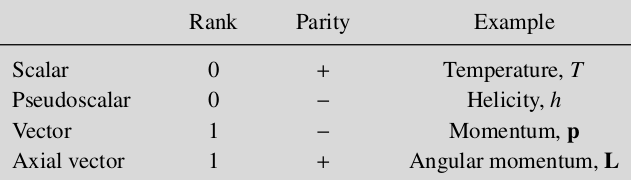
\includegraphics[width=\linewidth]{images/V-A.png}
\end{center}

Parity not conserved in weak interaction. Discovered by Wu, who saw $^{60}Co \to ^{60}Ni^* + e^- + \bar{\nu}_e$

\begin{center}
    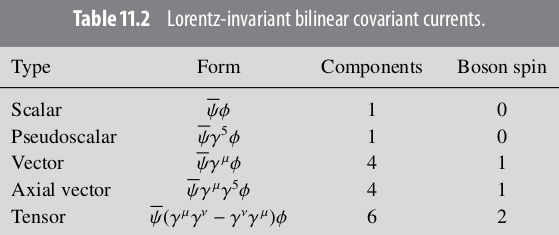
\includegraphics[width=\linewidth]{images/bilinear_covariant_currents.png}
\end{center}

Experimentally we found the interaction is V-A, with a vertex term $\frac{-ig_W}{\sqrt{2}}\frac{1}{2}\gamma^\mu(1 - \gamma^5)$.

\textbf{Weak Feynman Rules}

Fermions: same as before, same vibe with neutrinos

W / Z: same as photons for incoming/outgoing

W prop: $-\frac{i[g_{\mu\nu} - q_\mu q_\nu / m_W^2]}{q^2 - m_W^2}$

If $q^2$ small: $\frac{-ig_{\mu\nu}}{q^2 - m_W^2}$

If $q^2$ really small: $\frac{ig_{\mu\nu}}{m_W^2}$

Vertex: $\frac{-ig_w}{\sqrt{2}}\frac{1}{2}\gamma^\mu (1 - \gamma^5)$

For spin-0 kaons or pions, can replace $\bar{v}\gamma^\mu (1 - \gamma^5)u$ with $f_\pi p_\pi^\mu$

If $q^2$ small, $\frac{G_F}{\sqrt{2}} = \frac{g_W^2}{8m_W^2}$

(Fermi: assuming no W boson propagator $q^2$ dependence)

Because we have $V-A$, only LH chiral particles and RH chiral anti-particles participate in weak CC interactions.

Remember $u/c/t \to W \to d/s/b$ only.

\todo[inline]{More pion decay stuff?}
